
早期計算機的編程非常困難,因為處理器慢、內存有限、編譯器差勁,完成一個程序需要花費大量的時間。開發者必須知道CPU架構、內存佈局,對於當時的編譯器,關鍵的代碼必須用匯編來寫。

後來情況有所好轉了。處理器的速度越來越快,編譯器開發者可以使用了一些使程序更快的技巧,所以曾經需要巨大硬盤容量的處理器,現在的所需的容量也就一個普通PC機主存的大小,開發者可以花更多的時間來解決問題,這反映在編程語言和設計風格上。在高級語言和不斷髮展的設計和編程實踐之間,開發者的重點從想在代碼中\textbf{說什麼},轉變為想\textbf{怎麼說}。

以前的常識,如CPU到底有多少寄存器,寄存器的名字都是什麼,現在卻變成了深奧且難懂的話題。曾經的“大型代碼庫”很難進行管理,而現在已經完全在版本控制系統的掌握之下了。幾乎不需要為特定的處理器或內存系統編寫特定的代碼,可移植的代碼已經越來越流行了。

對於手動彙編編程,實際上很難超越編譯器生成的代碼。當代碼量增加,大多數開發者無法完成手動彙編。對於應用程序和編寫者來說,有“足夠的性能”即可,開發者需要對其他方面的事情更加關注(需要明確的是,開發者可以專注於代碼的可讀性,而不必擔心添加一個名稱有意義的函數是否會使程序慢)。

然後,也算是老生常談,“性能自增長”的時代結束了。看似不斷增長的計算能力的提升在程序性能方面……停止了。


\hspace*{\fill} \\ %插入空行
\begin{center}
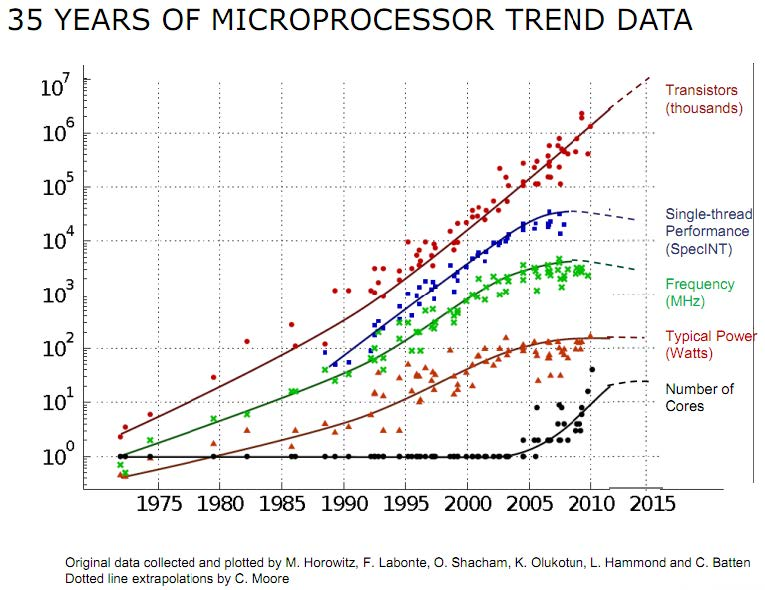
\includegraphics[width=0.9\textwidth]{content/1/chapter1/images/1.jpg}\\
圖1.1 -微處理器35年的發展歷程 \\
(引用於 \url{https://github.com/karlrupp/microprocessor-trend-data and https://github.com/karlrupp/microprocessor-trend-data/blob/master/LICENSE.txt})
\end{center}

2005年左右,單個CPU的計算能力達到飽和,CPU頻率也停止增長。CPU的頻率又受到幾個因素的限制,其中之一是功耗(如果頻率趨勢保持不變,如今的CPU每平方毫米的功率將超過將火箭送入太空的大型噴氣式發動機)。

從前面的圖表中可以明顯看出,並不是所有的進步指標都在2005年停滯不前:集成在單個芯片中的晶體管數量一直在增長。那麼,如果不是讓芯片更快,那是在做什麼呢?圖表下面的曲線揭示了其中的部分原因。設計師沒有將單個處理器做得更大,而是將多個處理器核心放在一起。當然,這些處理器的計算能力會隨著核的數量而增加。“晶體管之謎”的第二部分(晶體管都到哪裡去了?)中,硬件設計師對處理器功能進行了增強,可以用來提高性能,但也需要開發者瞭解如何使用。

處理器的變化是併發編程進入主流的原因,但這種變化的意義遠不止於此。本書中為了獲得最佳性能,開發者需要理解處理器和內存體系結構,及其間的交互,所以出色的性能不再是“偶然獲得”。與此同時,在編寫代碼時所取得的進步,也清楚地表達了需要做什麼,而不是如何做。我們仍然希望編寫可讀和可維護的代碼,並且(不是但是)這些代碼是高效的。

可以肯定的是,對於許多應用程序來說,現代CPU的性能已經足夠,但程序的性能比過去有了更多的關注,這在很大程度上是因為CPU的變化。因為我們想在不一定能獲得最佳計算資源的應用程序中,做更多的計算(例如,今天的便攜式醫療設備可能有一個神經網絡程序在其中工作)。

幸運的是,我們不必在黑暗的儲藏室裡翻找一堆堆腐爛的穿孔卡片,來重新學習那些古老的藝術形式。任何時候,都有困難的問題,對於許多軟件開發者來說,\textit{計算能力永遠不夠用}這句話完全正確。隨著計算能力呈指數級增長,對它的需求也在相應的增長(古老的藝術只會在少數需要它的領域中得以延續)。











